\documentclass{article}
\usepackage{titling}
\usepackage{lipsum}
\usepackage{amsmath}
\usepackage{listings}
\usepackage{graphicx}
\usepackage{subcaption}
\usepackage{pgfplots}
\usepackage[margin=1in]{geometry}
\usepgfplotslibrary{statistics}



\begin{document}
\noindent
\begin{minipage}[t]{0.6\textwidth}
    \begin{flushleft}
        \LARGE\textbf{Math 343 - Lab 7} \\
        \vspace{6pt} % add 6pt of vertical space
        \hrule width 10cm
        \vspace{12pt}
        \large\textbf{Preston Duffield} \\
        \large Western Washington University \\
        \today
        % April 18, 2023
        \vspace{24pt}
    \end{flushleft}
\end{minipage}

\section*{Question 1}
\subsection*{a)}
\begin{figure}[h]
    \centering
    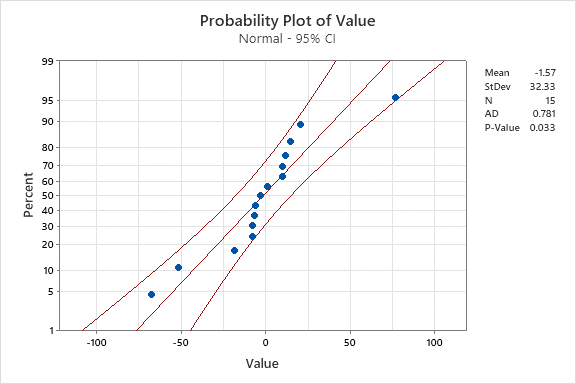
\includegraphics[width=0.8\textwidth]{./images/1_a.png}
    \caption{Normal Probability Plot from Minitab.}
    \label{fig:3_b_2}
\end{figure}

\subsection*{b)}
It would appear that only the effect of A is dominant.

\clearpage
\section*{Question 2}
\subsection*{a)}
\begin{figure}[h]
    \centering
    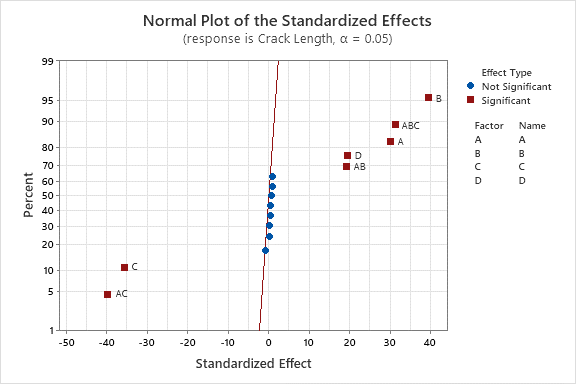
\includegraphics[width=0.8\textwidth]{./images/2_a.png}
    \caption{Normal Probability Plot from Minitab.}
    \label{fig:3_b_2}
\end{figure}
\subsection*{b)}
\begin{figure}[h]
    \centering
    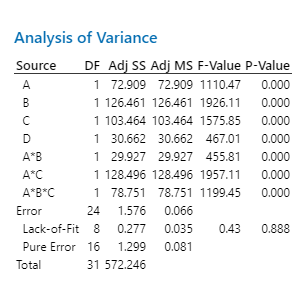
\includegraphics[width=0.4\textwidth]{./images/2_b.png}
    \caption{ANOVA Table from Minitab.}
    \label{fig:3_b_2}
\end{figure}
Since the p-value $< \alpha$ for each effect, they are all significant.
\clearpage
\subsection*{c)}
\begin{align*}
    SS_{Effect} &= \left(n2^{k-2}\right)\left(\text{Est. Effect}\right)^2 \\
                &= \left(2 \cdot 2^{4-2}\right)\left(\text{3.0189}\right)^2 \\
                &= 8 \cdot 9.11375721\\
                &= 72.91005768
\end{align*}
Yes this value is effectivly the same.
\subsection*{d)}
\begin{align*}
    -39.79 &\pm t_{\alpha/2, df_{error}} \cdot \sqrt{\frac{MSE}{n2^{k-2}}}\\
           &\pm t_{0.025, 24} \cdot \sqrt{\frac{0.066}{2 \cdot 2^{4-2}}}\\
           &\pm 2.064 \cdot \sqrt{\frac{0.066}{2 \cdot 2^{4-2}}}\\
           &\pm 2.064 \cdot \sqrt{0.00825}\\
           &\pm 0.1874721099
\end{align*}
We are 95\% confident that the true value of the main effect of AC is between -39.977, and -39.602.

\end{document}
